\chapter{Ontwikkelingsgenetica en de evolutie van de vorm}\label{ch:b3:developmental-genetics}

Het ei van een fruitvlieg is een halve millimeter lang, en in de drie
uur na de bevruchting, voordat er ook maar één celmembraan tussen zijn
zesduizend kernen is gevormd, beslist het welk uiteinde de kop wordt en
welk de staart, waar elk van de veertien segmenten komt te liggen, en
welke ervan poten, vleugels of antennen zullen dragen. Het doet dat met
enkele tientallen genen, die in een hiërarchie van steeds fijnere
strepen worden aangezet, waarbij elke streep wordt afgelezen uit de
concentraties van de producten van de strepen ervoor. In 1980
doorzochten twee jonge onderzoekers in Heidelberg duizenden gemuteerde
vliegen op larven met ontbrekende of verdubbelde delen, en vonden de
hele hiërarchie: genen wier verlies een blok segmenten wist, genen wier
verlies elk tweede segment wist, genen wier verlies elk segment
achterstevoren keert. Het werk van datzelfde jaar aan een gen dat het
derde segment van een vlieg in een kopie van het tweede verandert ---
waarmee zij vier vleugels krijgt, zoals haar voorouders --- opende een
reeks meestergenen die, zo bleek, in dezelfde volgorde op de
chromosomen van een muis en een mens liggen en hetzelfde werk doen. Dit
hoofdstuk gaat over hoe een embryo zijn eigen meetkunde berekent, hoe
een paar honderd regelgenen elk dierlijk lichaam bouwen, en hoe het
veranderen van wanneer en waar zij werken de verscheidenheid van de
dierlijke vorm heeft voortgebracht.

\section{De coördinaten van de vlieg}

\begin{definition}[De hiërarchie van de segmentatie]\label{def:b3:developmental-genetics:hierarchy}
\index{maternaal-effectgen}\index{gapgen}\index{paarregelgen}\index{segmentpolariteitsgen}\index{syncytiaal blastoderm}
Het embryo van \emph{Drosophila} ontwikkelt zich gedurende zijn eerste
dertien kerndelingen als een \emph{syncytiaal blastoderm}, één enkele
cel wier kernen één cytoplasma delen, zodat eiwitten vrij kunnen
diffunderen vanaf de plaats waar zij worden gemaakt. Vier gradiënten
die door de cellen van de moeder zijn aangelegd bepalen de assen: het
mRNA van \emph{bicoid} ligt vastgelegd aan de voorste pool en zijn
eiwit diffundeert naar achteren tot een exponentiële gradiënt van kop
naar staart; het mRNA van \emph{nanos} aan de achterste pool maakt de
spiegelgradiënt; de mRNA's van \emph{hunchback} en \emph{caudal} zijn
gelijkmatig verdeeld, maar het Bicoid-eiwit onderdrukt de translatie
van \emph{caudal} en Nanos onderdrukt \emph{hunchback}, zodat ook hun
eiwitten gradiënten vormen. Deze \emph{maternaal-effectproducten},
wier mutante verschijningsvorm van het genotype van de moeder afhangt
en niet van dat van het embryo, zetten de \emph{gapgenen}
(\emph{hunchback}, \emph{Krüppel}, \emph{knirps}, \emph{giant}) aan in
brede banden, die elk op een bereik van Bicoid-concentraties antwoorden
en hun buren onderdrukken; de gapeiwitten zetten, in combinatie, de
\emph{paarregelgenen} (\emph{even-skipped}, \emph{fushi tarazu},
\emph{hairy}) aan in zeven strepen elk, om en om; en de
paarregeleiwitten zetten de \emph{segmentpolariteitsgenen}
(\emph{engrailed}, \emph{wingless}, \emph{hedgehog}) aan in veertien
strepen, één per segment, die de voor- en achterkant van elk segment
vastleggen en, nadat de cellen zijn gevormd, door signalen tussen die
cellen in stand worden gehouden. Drie uur, vier lagen, van één gradiënt
tot veertien segmenten --- en de namen van de mutanten leggen de
zoektocht vast: \emph{hunchback} mist het borststuk, \emph{Krüppel}
(``kreupel'') het midden, \emph{fushi tarazu} (``niet genoeg
segmenten'') elk tweede segment, \emph{hedgehog} heeft een grasveld van
borstels.
\end{definition}

\begin{omfigure}
\begin{tikzpicture}[every node/.style={font=\scriptsize}, >=stealth]
  \foreach \y/\lab/\n in {0/{maternaal: Bicoid-gradiënt}/1, -1.3/{gapgenen: 4 brede banden}/2, -2.6/{paarregelgenen: 7 strepen}/3, -3.9/{segmentpolariteit: 14 strepen}/4} {
    \draw[thick, gray!60] (0,\y) ellipse (3.6 and 0.5);
    \node[left, align=right] at (-3.8,\y) {\lab};
  }
  % bicoid gradient shading
  \begin{scope}
    \clip (0,0) ellipse (3.6 and 0.5);
    \shade[left color=omDef!80, right color=omDef!2] (-3.6,-0.5) rectangle (3.6,0.5);
  \end{scope}
  \node[right, font=\tiny] at (3.7,0) {vooraan hoog};
  % gap bands
  \begin{scope}
    \clip (0,-1.3) ellipse (3.6 and 0.5);
    \fill[omDef!50] (-3.4,-1.8) rectangle (-1.6,-0.8); \fill[omThm!40] (-1.4,-1.8) rectangle (0.2,-0.8); \fill[omMeth!40] (0.4,-1.8) rectangle (1.7,-0.8); \fill[omProp!45] (1.9,-1.8) rectangle (3.4,-0.8);
  \end{scope}
  \node[font=\tiny] at (-2.5,-1.3) {\emph{hb}}; \node[font=\tiny] at (-0.6,-1.3) {\emph{Kr}}; \node[font=\tiny] at (1.05,-1.3) {\emph{kni}}; \node[font=\tiny] at (2.65,-1.3) {\emph{gt}};
  % pair-rule stripes
  \begin{scope}
    \clip (0,-2.6) ellipse (3.6 and 0.5);
    \foreach \i in {0,...,6} { \fill[omThm!50] ({-3.1+\i*0.9},-3.1) rectangle ({-2.75+\i*0.9},-2.1); }
  \end{scope}
  \node[right, font=\tiny] at (3.7,-2.6) {\emph{eve}, elk tweede segment};
  % segment polarity stripes
  \begin{scope}
    \clip (0,-3.9) ellipse (3.6 and 0.5);
    \foreach \i in {0,...,13} { \fill[omProp!60] ({-3.25+\i*0.47},-4.4) rectangle ({-3.1+\i*0.47},-3.4); }
  \end{scope}
  \node[right, font=\tiny] at (3.7,-3.9) {\emph{en}: één per segment};
  \foreach \y in {-0.55,-1.85,-3.15} { \draw[->, thick] (0,\y) -- (0,\y-0.2); }
  \node[below, align=center, font=\tiny] at (0,-4.5) {elke laag leest de concentraties van de laag erboven;\\drie uur van één gradiënt tot veertien segmenten};
\end{tikzpicture}

{\small De hiërarchie van de segmentatie. Een maternale gradiënt wordt
gelezen als vier banden van \omterm{def:b3:developmental-genetics:hierarchy}{gapgenen}; de gapeiwitten, in combinatie,
als zeven strepen van \omterm{def:b3:developmental-genetics:hierarchy}{paarregelgenen}; die weer als veertien strepen van
segmentpolariteit. Elke streep is een grens, getrokken waar een
concentratie een drempel passeert.}
\end{omfigure}

\begin{theorem}[Een morfogeengradiënt uit aanmaak, diffusie en afbraak]\label{thm:b3:developmental-genetics:gradient}
\index{morfogeen}\index{positie-informatie}\index{model van de Franse vlag}\index{vervallengte}
Een eiwit dat aan het ene uiteinde van een weefsel met snelheid $J$
(per oppervlakte-eenheid) wordt gemaakt, met coëfficiënt $D$
diffundeert en met snelheidsconstante $k$ wordt afgebroken, bereikt een
stationaire toestand waarin zijn concentratie langs de as $x$ voldoet
aan
\[
D\,\frac{\mathrm{d}^{2}c}{\mathrm{d}x^{2}} - k\,c = 0,
\qquad c(x) = c_{0}\,\mathrm{e}^{-x/\lambda}, \qquad \lambda = \sqrt{D/k},
\quad c_{0} = \frac{J}{\sqrt{Dk}} .
\]
De \emph{\omterm{thm:b3:developmental-genetics:gradient}{vervallengte}} $\lambda$ bepaalt hoe ver de gradiënt reikt; een
cel leest haar positie af door $c$ met drempels te vergelijken --- de
\emph{Franse vlag} van Wolpert (1969): boven $T_{1}$ blauw, tussen
$T_{1}$ en $T_{2}$ wit, eronder rood --- en de grens voor drempel
$T$ ligt bij $x_{T} = \lambda\ln(c_{0}/T)$. Twee gevolgen: de bron
verdubbelen verschuift elke grens met dezelfde $\lambda\ln 2$ naar
achteren, en een relatieve fout $\delta c/c$ bij het aflezen van de
concentratie is een positiefout $\delta x = \lambda\,\delta c/c$, zodat
een gradiënt een grens alleen tot op één cel nauwkeurig kan plaatsen
als de cellen haar tot op enkele procenten aflezen. Bicoid heeft
$\lambda \approx \qty{100}{\micro m}$ in een ei van
\qty{500}{\micro m}: de gradiënt overspant een factor $\mathrm{e}^{5}
\approx 150$, en de grens van \emph{hunchback} ligt halverwege het ei,
waar Bicoid tot ongeveer een twaalfde van zijn piek is gedaald.
\end{theorem}
\begin{proof}
Behoud in een schijf tussen $x$ en $x + \mathrm{d}x$: de netto
diffusieve instroom $D\,\partial^{2}c/\partial x^{2}$ is in de
stationaire toestand in evenwicht met de afbraak $kc$, wat de
vergelijking geeft; de oplossing die begrensd blijft als
$x \to \infty$ is de dalende e-macht met
$\lambda^{2} = D/k$. De bron: de diffusieve stroom bij $x = 0$, $-D\,
c'(0) = Dc_{0}/\lambda$, is gelijk aan $J$, dus $c_{0} = J\lambda/D =
J/\sqrt{Dk}$. Drempel: $c_{0}\mathrm{e}^{-x_{T}/\lambda} = T$ geeft
$x_{T}$; $c_{0}$ verdubbelen telt $\lambda\ln 2$ bij elke $x_{T}$ op,
ongeacht $T$. Fout: differentiëren van $x_{T} = \lambda\ln(c_{0}/c)$
geeft $\delta x = -\lambda\,\delta c/c$. De stationaire toestand wordt
bereikt op de tijdschaal $1/k$, die voor Bicoid (\qty{50}{min})
vergelijkbaar is met de twee uur die beschikbaar zijn, zodat de
gradiënt wordt afgelezen terwijl hij nog tot rust komt.
\end{proof}

\begin{omfigure}
\begin{tikzpicture}
\begin{axis}[
  width=0.7\linewidth, height=5.6cm,
  axis x line=bottom, axis y line=left,
  xmin=0, xmax=500, ymin=0, ymax=1.05,
  xlabel={afstand tot de voorste pool (\unit{\micro m})}, ylabel={Bicoid, relatief},
  xlabel style={font=\small, at={(axis description cs:0.5,-0.12)}, anchor=north}, ylabel style={font=\small},
  tick label style={font=\small}, xtick={0,100,250,400,500}, ytick={0.08,0.3,0.6,1},
  yticklabels={0.08,0.3,0.6,1},
  clip=false,
]
\fill[omDef!15] (axis cs:0,0) rectangle (axis cs:120,1.05);
\fill[gray!8] (axis cs:120,0) rectangle (axis cs:250,1.05);
\fill[omThm!12] (axis cs:250,0) rectangle (axis cs:500,1.05);
\addplot[very thick, omDef, domain=0:500, samples=100] {exp(-x/100)};
\addplot[thick, omDef!50, dashed, domain=66:500, samples=100] {2*exp(-x/100)};
\draw[dashed, gray] (axis cs:0,0.3) -- (axis cs:120,0.3) -- (axis cs:120,0);
\draw[dashed, gray] (axis cs:0,0.08) -- (axis cs:250,0.08) -- (axis cs:250,0);
\node[font=\scriptsize, anchor=south] at (axis cs:60,1.0) {kop};
\node[font=\scriptsize, anchor=south] at (axis cs:185,1.0) {borststuk};
\node[font=\scriptsize, anchor=south] at (axis cs:375,1.0) {achterlijf};
\node[font=\scriptsize, omDef, anchor=west] at (axis cs:255,0.35) {$c = c_{0}\,\mathrm{e}^{-x/\lambda}$, $\lambda = \qty{100}{\micro m}$};
\node[font=\scriptsize, omDef!70!black, anchor=west, align=left] at (axis cs:255,0.62) {gestreept: bron verdubbeld ---\\elke grens verschuift met $\lambda\ln 2 = \qty{69}{\micro m}$};
\node[font=\scriptsize, gray, anchor=north east] at (axis cs:118,0.29) {$T_{1}$};
\node[font=\scriptsize, gray, anchor=south west] at (axis cs:300,0.09) {$T_{2}$: \emph{hunchback} uit};
\end{axis}
\end{tikzpicture}

{\small De Franse vlag, getekend door een e-macht. Drempels op één
gradiënt verdelen het ei in gebieden; een sterkere bron schuift alle
grenzen met dezelfde afstand naar achteren, en dat is wat embryo's van
moeders met extra kopieën van \emph{bicoid} laten zien.}
\end{omfigure}

\begin{proof}[Bewijsmateriaal]
Nüsslein-Volhard en Wieschaus (1980) gaven vliegen een mutageen te
eten, kweekten de nakomelingen tot homozygotie en bekeken onder de
microscoop de cuticula van zo'n \num{27000} dode larven op ontbrekend
of herhaald patroon: ongeveer honderdtwintig genen, naar hun
verschijningsvorm gesorteerd in de klassen van de gap-, de paarregel-
en de \omterm{def:b3:developmental-genetics:hierarchy}{segmentpolariteitsgenen} --- een hiërarchie die zichtbaar was
voordat er ook maar één molecuul bekend was. Driever en
Nüsslein-Volhard (1988) kleurden embryo's voor het Bicoid-eiwit en
zagen de exponentiële gradiënt vanaf de voorste pool; embryo's van
moeders met één, twee, vier of zes kopieën van het gen hadden
gradiënten met een evenredige hoogte, en de kopplooi en de grens van
\emph{hunchback} verschoven met de dosis naar achteren, zoals het
drempelmodel voorspelt en ruwweg met de $\lambda\ln 2$ per verdubbeling
die het vereist. Het mRNA van \emph{bicoid} in het midden van een ei
spuiten leverde daar een kop op.
\end{proof}

\begin{omfigure}
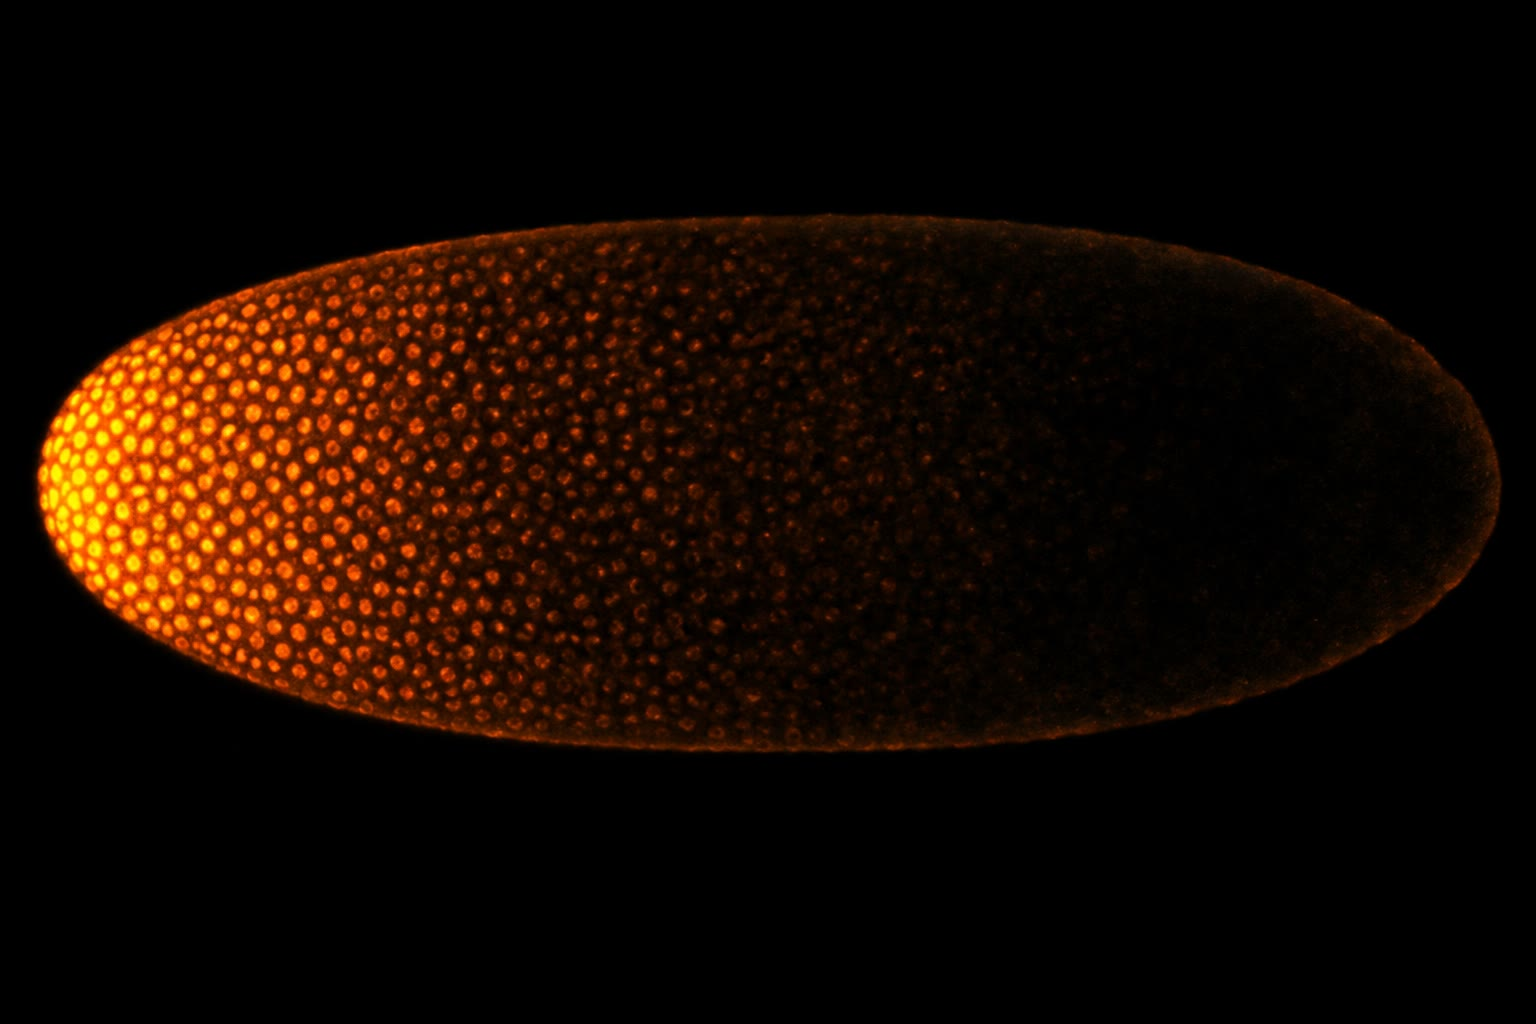
\includegraphics[width=0.46\linewidth]{images/book5/ai/b5-23-bicoid-gradient.jpg}\hspace{0.04\linewidth}
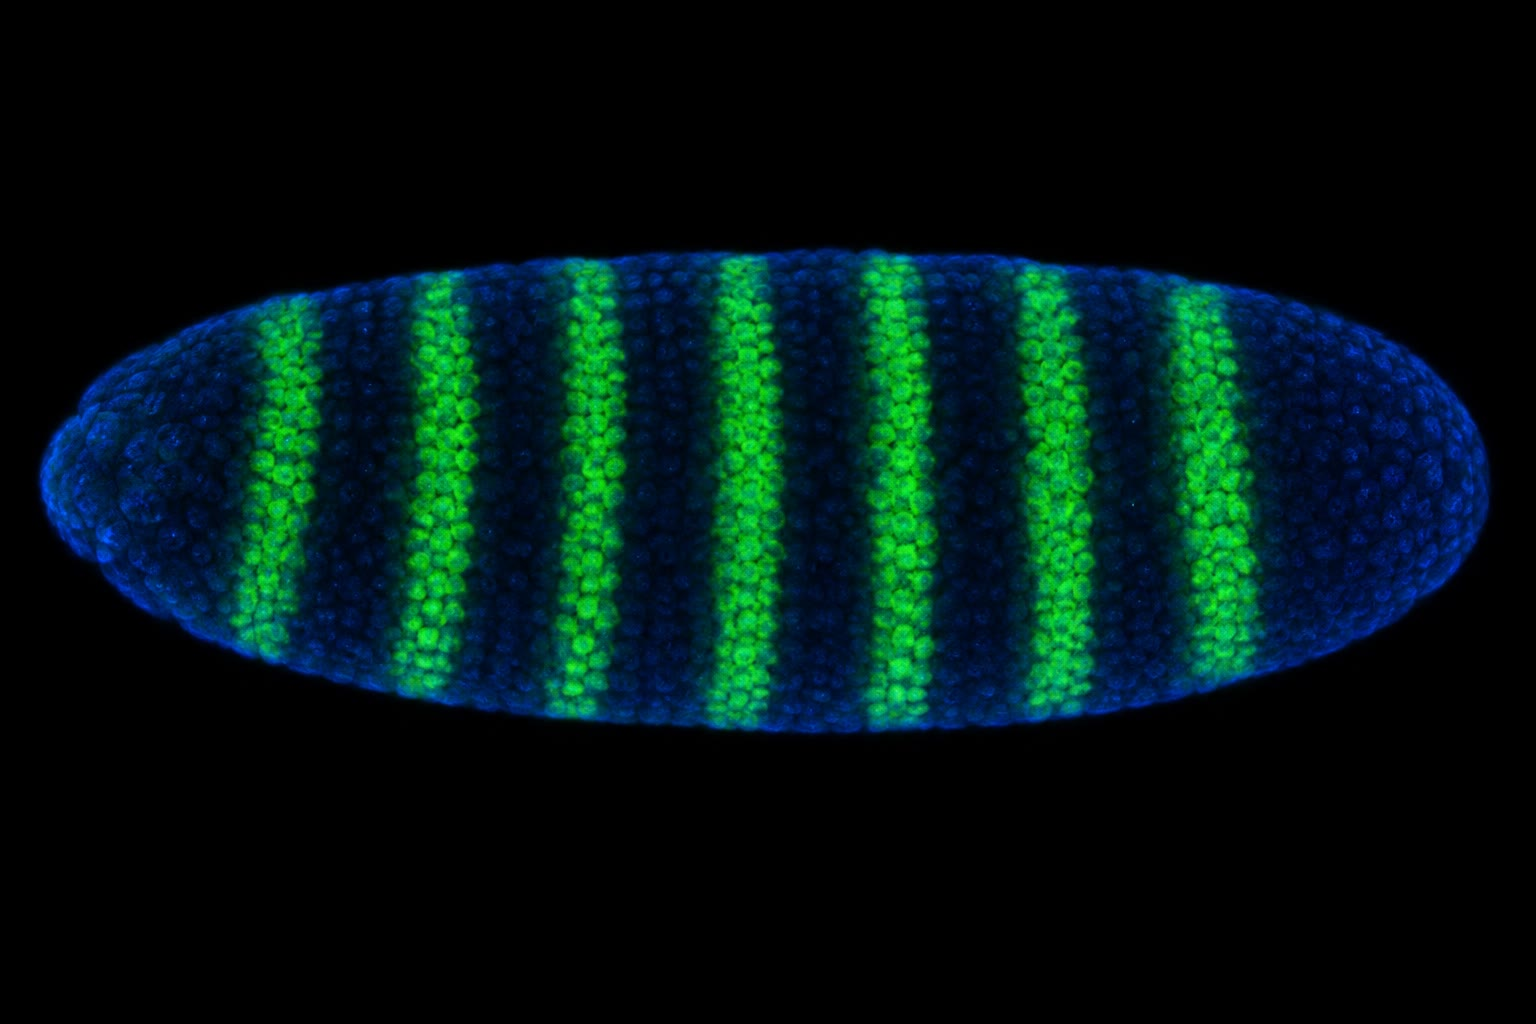
\includegraphics[width=0.46\linewidth]{images/book5/ai/b5-23-embryo-stripes.jpg}

{\small Links: een syncytiaal embryo gekleurd voor het Bicoid-eiwit,
het helderst aan de voorste pool en exponentieel wegdovend naar
achteren. Rechts: een embryo een uur later, gekleurd voor een
paarregeleiwit, zeven strepen getekend naar de banden van de \omterm{def:b3:developmental-genetics:hierarchy}{gapgenen}.}
\end{omfigure}

\section{Identiteit: de Hox-genen}

\begin{definition}[Homeotische genen en colineariteit]\label{def:b3:developmental-genetics:hox}
\index{homeotische mutatie}\index{Hox-genen}\index{colineariteit}\index{homeobox}\index{Hox-code}
Een \emph{homeotische} mutatie verandert het ene lichaamsdeel in het
andere: het woord van Bateson (1894) voor de afwijkingen die ``het ene
lid van een reeks door een ander vervangen''. Bij de vlieg laten
dominante mutanten van \emph{Antennapedia} poten groeien waar antennen
horen; mutanten van \emph{bithorax} (Lewis, 1978) veranderen het derde
borstsegment in een kopie van het tweede, zodat de halters een tweede
paar vleugels worden. De acht genen die daarvoor verantwoordelijk zijn,
de \emph{Hox-genen}, liggen in twee clusters op één chromosoom, en
Lewis merkte op dat hun volgorde op het DNA overeenkomt met de volgorde
langs het lichaam van de segmenten die zij besturen --- de
\emph{colineariteit}, die nog altijd niet volledig is verklaard. Elk
codeert een transcriptiefactor met hetzelfde DNA-bindende
\emph{homeobox}-domein van 60 aminozuren (McGinnis, Gehring, 1984), dat
daarna in elk dier werd gevonden: muizen en mensen dragen vier clusters
van elk dertien genen, op dezelfde wijze colineair, tot expressie
gebracht in geneste gebieden langs de lichaamsas, waarbij de latere
genen in het cluster verder naar achteren liggen. De identiteit van een
cel langs de as wordt gegeven door de combinatie van Hox-genen die zij
tot expressie brengt, de \emph{Hox-code}; achterste genen overheersen
voorste (achterste overwicht), zodat het verliezen van een achterste
gen het segment de identiteit van het segment ervoor laat aannemen.
Hox-genen bouwen geen segment; zij vertellen een reeds gebouwd segment
welk segment het is, door de batterijen van stroomafwaartse genen aan
te zetten die bij een poot, een vleugel, een rib of een lendenwervel
horen.
\end{definition}

\begin{omfigure}
\begin{tikzpicture}[every node/.style={font=\scriptsize}, >=stealth]
  % fly cluster
  \node[left] at (-0.3,2.2) {vlieg (\emph{Drosophila}), 8 genen};
  \foreach \i/\g/\c in {0/lab/omDef, 1/pb/omDef, 2/Dfd/omThm, 3/Scr/omThm, 4/Antp/omMeth, 5/Ubx/omMeth, 6/abd-A/omProp, 7/Abd-B/omProp} {
    \draw[thick, fill=\c!40] ({\i*1.1},1.9) rectangle ({\i*1.1+0.9},2.5); \node[font=\tiny] at ({\i*1.1+0.45},2.2) {\emph{\g}};
  }
  \node[left] at (-0.3,0.9) {HoxB-cluster van de muis, 9 van 13};
  \foreach \i/\g/\c in {0/b1/omDef, 1/b2/omDef, 2/b3/omDef, 3/b4/omThm, 4/b5/omThm, 5/b6/omMeth, 6/b7/omMeth, 7/b8/omProp, 8/b9/omProp} {
    \draw[thick, fill=\c!40] ({\i*1.1},0.6) rectangle ({\i*1.1+0.9},1.2); \node[font=\tiny] at ({\i*1.1+0.45},0.9) {\emph{\g}};
  }
  \draw[->, thick] (0,1.55) -- (9.8,1.55); \node[above, font=\tiny] at (4.9,2.55) {3$'$ $\to$ 5$'$ langs het DNA};
  \draw[->, thick] (0,0.2) -- (9.8,0.2); \node[below, font=\tiny] at (4.9,0.05) {voor $\to$ achter langs het lichaam};
  % body schematic
  \node[left] at (-0.3,-0.9) {tot expressie in};
  \draw[thick, gray!70, rounded corners=6pt] (0,-1.3) rectangle (9.8,-0.5);
  \foreach \x/\t in {0.6/kop, 2.6/nek, 4.4/borststuk, 6.6/lende, 8.6/{sacraal, staart}} { \node[font=\tiny] at (\x,-0.9) {\t}; }
  \draw[gray!70] (1.6,-1.3) -- (1.6,-0.5); \draw[gray!70] (3.5,-1.3) -- (3.5,-0.5); \draw[gray!70] (5.6,-1.3) -- (5.6,-0.5); \draw[gray!70] (7.6,-1.3) -- (7.6,-0.5);
  \node[below, align=center, font=\tiny] at (4.9,-1.4) {colineariteit: de volgorde van de genen op het chromosoom is de volgorde van hun gebieden langs het lichaam;\\dezelfde clusters, dezelfde volgorde, van vlieg tot muis ---\\geërfd van een voorouder van 600 miljoen jaar geleden};
\end{tikzpicture}

{\small Hox-clusters bij een vlieg en een muis. De genen liggen op het
DNA in de volgorde van de lichaamsgebieden die zij vastleggen, bij
beide dieren, en de homologe genen zijn aan hun sequentie te herkennen:
het gen \emph{Hoxb6} van een muis is herkenbaar het
\emph{Antennapedia} van de vlieg.}
\end{omfigure}

\begin{proof}[Bewijsmateriaal]
Lewis (1978) bracht het \emph{bithorax}-complex in kaart als een reeks
mutaties die elk één segment in het segment ervoor veranderden, op het
chromosoom in de volgorde van het lichaam gerangschikt, en stelde voor
dat de genen langs de as achtereenvolgens werden geactiveerd. McGinnis
en collega's (1984) vonden de \omterm{def:b3:developmental-genetics:hox}{homeobox} door kruishybridisatie tussen
\emph{Antennapedia} en \emph{Ultrabithorax} en daarna in kikkers en
muizen. De functionele gelijkwaardigheid werd rechtstreeks aangetoond:
een gen \emph{Hoxb6} van een muis dat in een vlieg tot expressie wordt
gebracht geeft de verschijningsvorm van \emph{Antennapedia}, poten uit
antennen (jaren 1990); een muis zonder \emph{Hoxc8} heeft een extra rib
op haar eerste lendenwervel, omdat dat segment de identiteit van het
segment ervoor heeft aangenomen; en het verschuiven van de
expressiegrenzen van Hox bij kip en muis verplaatst de plek waar de
voorpoten ontstaan, waarbij de lengte van de nek van een zwaan wordt
geëvenaard door een verschuiving van dezelfde grens naar achteren.
\end{proof}

\begin{omfigure}
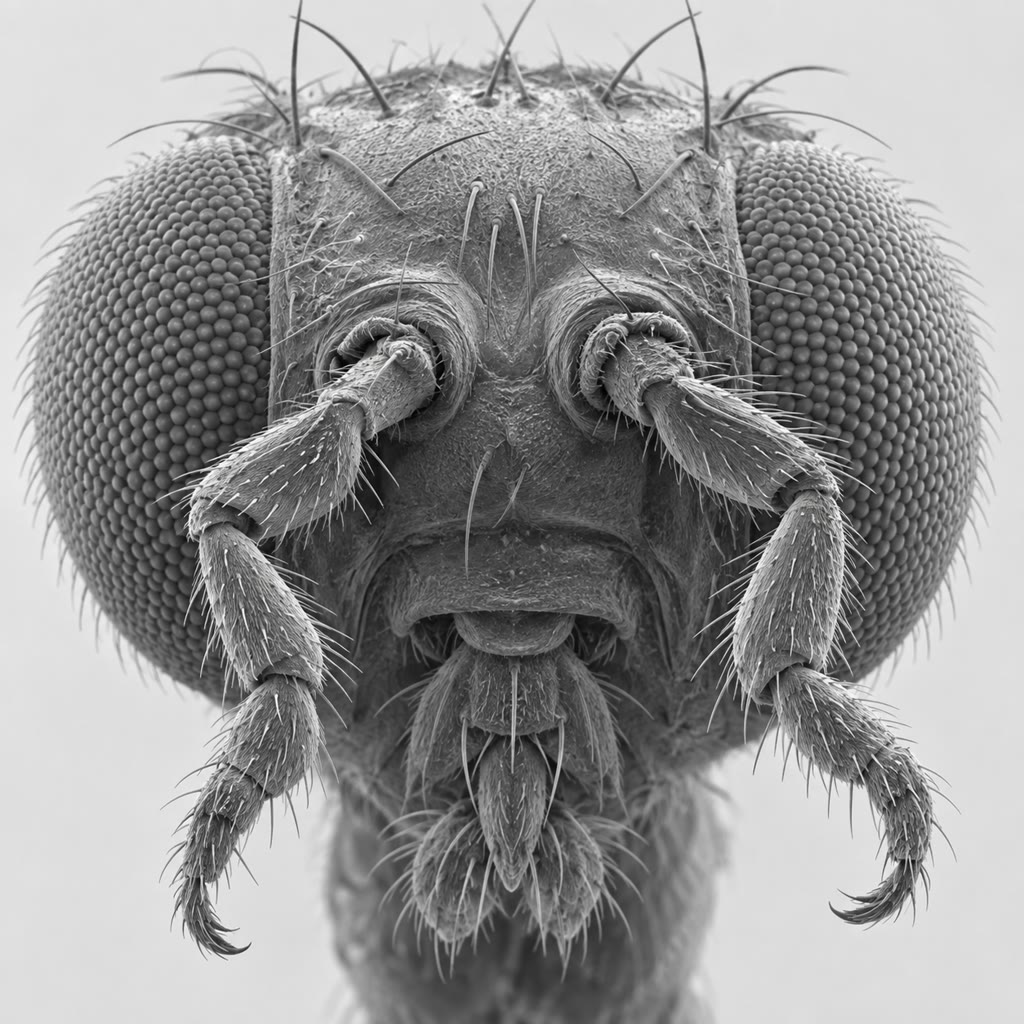
\includegraphics[width=0.34\linewidth]{images/book5/ai/b5-23-antennapedia-fly.jpg}\hspace{0.04\linewidth}
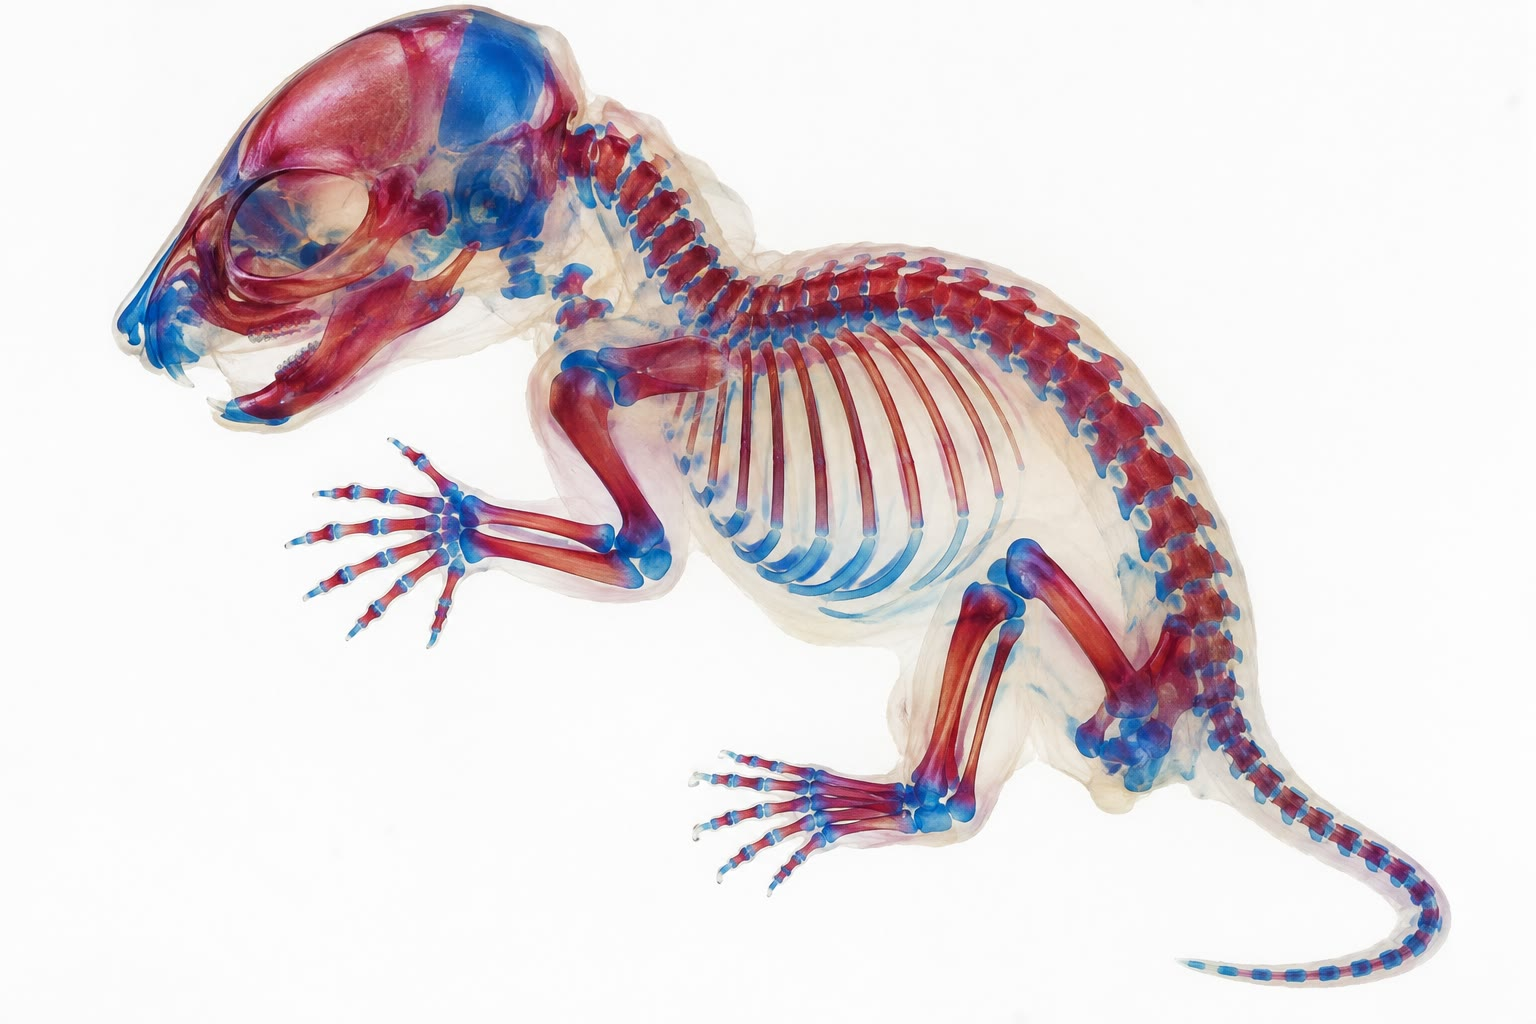
\includegraphics[width=0.5\linewidth]{images/book5/ai/b5-23-limb-skeleton-stain.jpg}

{\small Links: de kop van een vlieg met de mutatie
\emph{Antennapedia}, een paar poten waar de antennen horen --- het
segment is correct gebouwd en heeft de verkeerde identiteit gekregen.
Rechts: het skelet van een muizenembryo, kraakbeen blauw en bot rood,
de wervels waarlangs de \omterm{def:b3:developmental-genetics:hox}{Hox-code} wordt gelezen.}
\end{omfigure}

\section{Een gewervelde bouwen}

\begin{definition}[Organisatoren en signaalcentra]\label{def:b3:developmental-genetics:organiser}
\index{organisator}\index{inductie}\index{sonic hedgehog}\index{ledemaatknop}\index{zone van polariserende activiteit}\index{apicale ectodermale lijst}
Embryo's van gewervelden bestaan vanaf het begin uit cellen, dus worden
hun gradiënten gemaakt door uitgescheiden eiwitten in plaats van door
diffusie in een syncytium, en dezelfde paar families doen alles: Wnt,
Hedgehog, BMP en andere verwanten van TGF-$\beta$, FGF, Notch en
retinoïnezuur. Spemann en Mangold (1924) plaatsten een stukje van de
rugzijdige lip van een gastrula van een watersalamander op de buik van
een andere en verkregen een tweede embryo, van kop tot staart,
grotendeels uit cellen van de gastheer: het transplantaat was een
\emph{organisator}, die zijn buren tot het vormen van een zenuwstelsel
en een as aanzette, en zeventig jaar later bleken zijn moleculen
uitgescheiden tegenspelers (Chordin, Noggin) te zijn die BMP blokkeren,
wier afwezigheid het ectoderm neuraal laat worden --- de
standaardkeuze. De \emph{neurale buis} wordt daarna van rug naar buik
gepatroneerd door \emph{sonic hedgehog} uit de chorda en de bodemplaat
(veel: motorneuronen; weinig: \omterm{def:b3:nervous-systems:cells}{interneuronen}) tegen BMP van het dak; en
de \emph{ledemaatknop} door twee centra, de \emph{zone van
polariserende activiteit} aan de achterrand, die Shh uitscheidt (een
transplantaat ervan naar de voorrand geeft een spiegelbeeldige
verdubbeling van de vingers, zes vingers die duim tegen duim staan), en
de \emph{apicale ectodermale lijst} aan de top, die FGF's uitscheidt
die de cellen eronder aan het delen houden en de volgorde van
opperarmbeen, onderarm en hand van binnen naar buiten vastleggen.
Transplanteren, wegnemen en in eiwit gedrenkte bolletjes blijven het
gereedschap; de logica --- een plaatselijke bron, een gradiënt,
drempels, een code van transcriptiefactoren --- is die van de vlieg.
\end{definition}

\begin{omfigure}
\begin{tikzpicture}[every node/.style={font=\scriptsize}, >=stealth]
  % limb bud
  \fill[omDef!12] (0,0) -- (0,3) .. controls (2.6,3.4) and (3.4,2.2) .. (3.4,1.5) .. controls (3.4,0.8) and (2.6,-0.4) .. (0,0) -- cycle;
  \draw[thick, omDef] (0,0) -- (0,3) .. controls (2.6,3.4) and (3.4,2.2) .. (3.4,1.5) .. controls (3.4,0.8) and (2.6,-0.4) .. (0,0);
  \draw[very thick, omMeth!70!black] (2.9,2.5) .. controls (3.45,1.9) and (3.45,1.1) .. (2.9,0.5);
  \node[right, align=left, omMeth!70!black, font=\tiny] at (3.5,1.5) {apicale ectodermale lijst:\\FGF8; houdt de\\voortgangszone aan het delen;\\proximaal $\to$ distaal};
  \begin{scope}
    \clip (0,0) -- (0,3) .. controls (2.6,3.4) and (3.4,2.2) .. (3.4,1.5) .. controls (3.4,0.8) and (2.6,-0.4) .. (0,0) -- cycle;
    \foreach \i/\op in {1/50, 2/38, 3/26, 4/14} { \draw[omThm!\op, thick] (0.6,0.5) circle ({0.45*\i}); }
  \end{scope}
  \fill[omThm!50] (0.6,0.5) ellipse (0.5 and 0.35); \node[anchor=north, align=center, omThm, font=\tiny] at (0.9,-0.2) {ZPA: sonic hedgehog,\\achter $\to$ voor};
  \node[left, font=\tiny] at (-0.05,2.6) {voor}; \node[left, font=\tiny] at (-0.05,0.4) {achter};
  \node[left, font=\tiny] at (-0.05,1.5) {lichaamswand};
  \draw[->, thick] (0.3,1.5) -- (3.0,1.5); \node[above, font=\tiny] at (1.75,1.55) {opperarmbeen, onderarm, vingers};
  % right: digit code
  \node[right, align=left] at (7.2,2.6) {vingeridentiteit naar blootstelling aan Shh:\\duim (vinger 1): geen;\\vingers 2--3: gradiënt;\\vingers 4--5: uit cellen die Shh maken};
  \node[right, align=left] at (7.2,1.0) {plaats vooraan een tweede ZPA:\\spiegelbeeldige verdubbeling, 4-3-2-2-3-4;\\een bolletje Shh-eiwit doet hetzelfde};
  \node[right, align=left, gray] at (7.2,-0.2) {hetzelfde molecuul patroneert de neurale buis\\(motorneuronen waar het hoog is) en de darm};
\end{tikzpicture}

{\small De twee signaalcentra van de \omterm{def:b3:developmental-genetics:organiser}{ledemaatknop}. \omterm{def:b3:developmental-genetics:organiser}{Sonic hedgehog} van
de achterrand vertelt cellen welke vinger zij moeten worden; FGF van de
top vertelt hun hoe ver naar buiten langs het ledemaat zij zitten.
Transplantaten die een centrum verplaatsen verplaatsen het patroon mee.}
\end{omfigure}

\begin{proposition}[Spontaan patroon: het mechanisme van Turing]\label{prop:b3:developmental-genetics:turing}
\index{Turing-patroon}\index{reactie--diffusie}\index{activator--remmer}
Niet elk patroon wordt uit een reeds bestaande gradiënt gelezen. Turing
(1952) toonde aan dat twee diffunderende stoffen die reageren --- een
\emph{activator} die zijn eigen aanmaak en die van een \emph{remmer}
prikkelt, en een remmer die de activator onderdrukt en veel sneller
diffundeert --- een gelijkmatig veld spontaan in een regelmatige reeks
pieken kunnen veranderen: een kleine plaatselijke overmaat aan
activator groeit door zelfversterking terwijl de remmer die hij
voortbrengt zich uitspreidt en verhindert dat er vlakbij nieuwe pieken
ontstaan, zodat de pieken verschijnen met een afstand die door het
bereik van de remmer wordt bepaald,
$\lambda \sim \sqrt{D_{\text{inh}}/k_{\text{inh}}}$, en niet door een
uitwendige coördinaat. Het mechanisme, waarvan de wiskunde hier wordt
aangenomen, is de beste verklaring voor de vlekken en strepen van
dierenvachten, de afstand tussen haarzakjes en verenknoppen, de richels
van het verhemelte, de vingers van de hand (wier aantal stijgt wanneer
de golflengte van het patroon wordt verkort door de Hox-activiteit te
verlagen), en de strepen van de zebravis, waar de wisselwerkende cellen
--- pigmentcellen die buren van de ene soort afstoten en die van een
andere op afstand aantrekken --- zijn aangewezen en hun strepen zich na
wegbranden met een laser precies zoals de theorie voorspelt opnieuw
hebben gevormd.
\end{proposition}
\admitted

\section{De evolutie van de vorm}

\begin{definition}[Evo-devo]\label{def:b3:developmental-genetics:evodevo}
\index{diepe homologie}\index{genetische gereedschapskist}\index{cis-regulatoire evolutie}\index{heterochronie}
De genen die dieren bouwen vormen een oude en gedeelde
\emph{gereedschapskist}: een paar honderd transcriptiefactoren en
signaalroutes die al in de gemeenschappelijke voorouder van alle dieren
aanwezig waren, en de verscheidenheid van de dieren komt vooral voort
uit veranderingen in \emph{wanneer, waar en hoeveel} zij tot expressie
komen en niet in wat zij coderen. \emph{Diepe homologie}: het gen
\emph{Pax6} stuurt de vorming van het oog bij vliegen, inktvissen en
muizen, wier ogen als organen niet homoloog zijn --- een \emph{Pax6}
van een muis dat op de poot van een vlieg tot expressie komt maakt daar
een extra vliegenoog (Halder, Gehring, 1995). \emph{Cis-regulatoire
evolutie}: het verlies van bekkenstekels bij stekelbaarzen in zoet
water is de verwijdering van één versterker van het gen \emph{Pitx1},
terwijl het eiwit onaangeroerd blijft en elders nog dienst doet; het
verlies van vleugelvlekken bij sommige fruitvliegen is een verandering
in een versterker van \emph{yellow}; het verlies van poten bij slangen
een kapotte versterker van \emph{\omterm{def:b3:developmental-genetics:organiser}{sonic hedgehog}} in het ledemaat.
\emph{Verschuivingen van Hox}: de grens van de expressie van
\emph{Hoxc6} markeert bij muis, kip, gans en slang gelijkelijk de
eerste borstwervel, bij wervel 7, 14, 23 en 3; het verlies van poten op
het achterlijf bij insecten was het Hox-eiwit Ubx dat een onderdrukkend
domein verwierf dat het potengen \emph{Distal-less} uitzet, terwijl het
dat bij kreeftachtigen niet doet. \emph{Heterochronie}, een verandering
in de tijdsordening van een ontwikkelingsprogramma, maakte van de
axolotl een blijvende larve en van het menselijke gezicht dat van een
jonge mensaap. De oude vraag hoe nieuwe vormen ontstaan wordt een vraag
over regelend DNA: het grootste deel van het genoom dat voor de vorm
telt is geen gen maar schakelaar.
\end{definition}

\begin{example}[Vier vleugels]\label{ex:b3:developmental-genetics:four-wings}
De voorouders van de vliegen hadden vier vleugels, zoals libellen en
bijen nog altijd; vliegen hebben er twee, met het achterste paar
teruggebracht tot de halters. Bij vliegen komt \emph{Ultrabithorax} in
het derde borstsegment tot expressie en onderdrukt daar het
vleugelprogramma --- een honderdtal doelgenen, waarbij een halter een
vleugel is met die genen uitgezet. De drievoudige mutant van Lewis, die
in het derde segment geen werkzaam \emph{Ubx} heeft, laat een tweede
paar vleugels groeien: geen nieuwe structuur maar het vrijkomen van een
oude. Bij vlinders komt \emph{Ubx} ook in de achtervleugel tot
expressie, en daar onderdrukt het de vleugel niet maar verandert het
haar patroon: hetzelfde eiwit, een andere verzameling doelwitten.
Vierhonderd miljoen jaar evolutie van de tweevleugeligen hing af van de
beslissing van één gen in één segment, en één mutatie draait haar in
één generatie terug --- en daarom is de geschiedenis van de vorm
leesbaar in de genen die haar bouwen.
\end{example}

\begin{remark}[Meetkunde uit chemie]\label{rem:b3:developmental-genetics:remark}
Een embryo heeft geen bouwtekening en geen landmeter. Het heeft een
paar gradiënten die door diffusie en afbraak worden gemaakt, cellen die
ze tegen drempels aflezen en transcriptiefactoren aanzetten, en een
code van die factoren die elk gebied vertelt wat het moet worden; het
heeft plaatselijke \omterm{def:b3:developmental-genetics:organiser}{organisatoren} die hun buren aanzetten, en reacties
die zichzelf patroneren. De wiskunde is die van de eerste-ordekinetiek
en de diffusie --- een e-macht, een vierkantswortel, een drempel --- en
zij verklaart niet alleen hoe de kop van een vlieg wordt geplaatst,
maar ook waarom een gen verdubbelen een grens over een vaste afstand
verschuift, waarom er zes vingers verschijnen wanneer een signaal wordt
verdubbeld, en waarom een slang driehonderd ribben heeft. De evolutie
bewerkt de schakelaars, niet de machine: de gereedschapskist van een
spons en die van een mens zijn vrijwel gelijk, en wat verschilt is de
bedrading.
\end{remark}

\section{Opgaven}

\begin{exercise}[$\star$]\label{exo:b3:developmental-genetics:1}
Noem de vier lagen van de segmentatiehiërarchie van de vlieg, van elk
één gen, en de verschijningsvorm van de mutant die het in zijn klasse
plaatste.
\end{exercise}

\begin{exercise}[$\star$]\label{exo:b3:developmental-genetics:2}
Wat is een \omterm{def:b3:developmental-genetics:hierarchy}{maternaal-effectgen}? Een vrouwtje dat homozygoot is voor een
nulmutatie van \emph{bicoid} wordt met een wildtype mannetje gepaard:
beschrijf haar embryo's en leg uit waarom hun eigen genotype hen niet
redt.
\end{exercise}

\begin{exercise}[$\star$]\label{exo:b3:developmental-genetics:3}
Formuleer de \omterm{def:b3:developmental-genetics:hox}{colineariteit} en het achterste overwicht. Voorspel de
verschijningsvorm van een muis zonder \emph{Hoxc8} en van een vlieg die
\emph{Antennapedia} in haar kop tot expressie brengt.
\end{exercise}

\begin{exercise}[$\star$]\label{exo:b3:developmental-genetics:4}
Wat toonde het transplantaat van Spemann en Mangold aan, en welke
moleculen bleken die van de \omterm{def:b3:developmental-genetics:organiser}{organisator} te zijn? Waarom heet het
neurale lot de ``standaardkeuze''?
\end{exercise}

\begin{exercise}[$\star\star$]\label{exo:b3:developmental-genetics:5}
Bicoid: $D = \qty{4}{\micro m^2/s}$, halveringstijd \qty{35}{min}.
Bereken $k$, $\lambda$, en de verhouding van de concentraties aan de
voorste pool en halverwege het ei (\qty{250}{\micro m}).
\end{exercise}

\begin{exercise}[$\star\star$]\label{exo:b3:developmental-genetics:6}
Met $\lambda = \qty{100}{\micro m}$ ligt een grens op
\qty{240}{\micro m}. Waar ligt zij als de moeder vier kopieën van
\emph{bicoid} draagt in plaats van twee? En bij één kopie? Druk de
verschuivingen uit als fractie van een ei van \qty{500}{\micro m}.
\end{exercise}

\begin{exercise}[$\star\star$]\label{exo:b3:developmental-genetics:7}
Kernen liggen in het blastoderm \qty{8}{\micro m} uiteen. Hoe
nauwkeurig moet een kern de Bicoid-concentratie aflezen om met
$\lambda = \qty{100}{\micro m}$ een grens tot op één kern te plaatsen?
Als de kern gedurende een tijd $\tau$ moleculen telt en de telling
Poisson-verdeeld is, hoeveel moet zij er dan tellen?
\end{exercise}

\begin{exercise}[$\star\star$]\label{exo:b3:developmental-genetics:8}
De gradiënt nadert de stationaire toestand op de tijdschaal $1/k$. Welk
deel van de stationaire concentratie is bij een halveringstijd van
\qty{35}{min} bereikt na \qty{60}{min}, \qty{90}{min} en
\qty{120}{min}? Wat betekent dat voor een embryo dat de gradiënt vóór
\qty{150}{min} moet aflezen?
\end{exercise}

\begin{exercise}[$\star\star$]\label{exo:b3:developmental-genetics:9}
Er wordt een ZPA op de voorrand van een \omterm{def:b3:developmental-genetics:organiser}{ledemaatknop} van een kip
geplaatst. Voorspel het vingerpatroon, en het patroon als er in plaats
daarvan een bolletje wordt ingebracht dat een lage dosis Shh afgeeft.
\end{exercise}

\begin{exercise}[$\star\star\star$]\label{exo:b3:developmental-genetics:10}
Een morfogeen wordt in een weefsel van lengte $L$ overal met snelheid
$s$ per volume-eenheid gemaakt, met snelheid $k$ afgebroken, en aan de
rand $x =
L$ vernietigd (een absorberende put), zonder stroom bij $x = 0$. Los
$Dc'' - kc + s =
0$ op voor $c(x)$ en schets het resultaat. Waarin verschilt de vorm van
deze gradiënt van die met een bron aan één uiteinde, en wat gebeurt er
als $L \ll \lambda$?
\end{exercise}

\begin{exercise}[$\star\star\star$]\label{exo:b3:developmental-genetics:11}
Twee drempels bij $T_{1} = 0.3c_{0}$ en $T_{2} = 0.08c_{0}$ verdelen
een gradiënt in drie gebieden. Toon aan dat de breedten van de eerste
twee gebieden niet van $c_{0}$ afhangen, en leg uit waarom een embryo
wiens \emph{lengte} van individu tot individu varieert (\qty{450}{} tot
\qty{550}{\micro m}) meer nodig heeft dan één e-macht om zijn patroon
mee te schalen. Stel één mechanisme voor.
\end{exercise}

\begin{exercise}[$\star\star\star$]\label{exo:b3:developmental-genetics:12}
Stekelbaarzen verloren hun bekkenstekels door een versterker van
\emph{Pitx1} te verwijderen, slangen verloren hun ledematen door een
versterker van \emph{\omterm{def:b3:developmental-genetics:organiser}{sonic hedgehog}} te breken. Leg uit waarom
veranderingen in de regeling en niet in de codering de gebruikelijke
weg zijn naar een verloren of veranderde structuur, in termen van
pleiotropie en van wat hetzelfde eiwit elders doet.
\end{exercise}

\section{Vraagstuk: de Franse vlag}

\begin{problem}[{Weekendvraagstuk --- het coördinatenstelsel van een ei
berekend uit eerste-ordekinetiek: de lengte van de Bicoid-gradiënt,
zijn bron en de tijd om te ontstaan, de grenzen die hij trekt en hun
nauwkeurigheid, wat de gendosis en de eigrootte ermee doen, en de
Hox-code die stroomafwaarts wordt gelezen, eindigend bij de
vervallengte, de verschuiving per verdubbeling en de nauwkeurigheid van
de positie}]
\label{pb:b3:developmental-genetics:1}
Gegevens: eilengte \qty{500}{\micro m}; Bicoid $D = \qty{4}{\micro m^2/s}$,
halveringstijd \qty{35}{min}; een bronstroom zo dat $c_{0} = \qty{50}{nM}$
bij twee maternale kopieën; afstand tussen de kernen
\qty{8.5}{\micro m} in cyclus 14; drempels $T_{1} = 0.3\,c_{0}$
(kop/borststuk) en $T_{2} =
0.08\,c_{0}$ (grens van \emph{hunchback}) voor het geval met twee
kopieën. Afleesruis $\delta c/c = 0.1$ voor één kern. Het getal van
Avogadro \qty{6e23}{}; een kern is een bol met straal \qty{3}{\micro m}.

\medskip
\noindent\textbf{Deel I --- De gradiënt.}
\begin{enumerate}
  \item Bereken $k$ uit de halveringstijd, in \unit{s^{-1}}, en de
        levensduur $1/k$ in minuten.
  \item Bereken $\lambda = \sqrt{D/k}$ in micrometer. Hoeveel
        \omterm{thm:b3:developmental-genetics:gradient}{vervallengten} is het ei?
  \item Met welke factor daalt de concentratie van pool tot pool? Met
        welke factor over één kernafstand halverwege het ei?
  \item Bereken de bronstroom $J = c_{0}\sqrt{Dk}$ in
        \unit{nM\,\micro m\,s^{-1}}, en het aantal moleculen dat per
        seconde een vlakje van \qty{1}{\micro m^2} van de voorste pool
        binnenkomt.
  \item Het aantal Bicoid-moleculen in een kern aan de pool ($c_{0}$)
        en halverwege het ei.
  \item Het deel van de stationaire toestand dat is bereikt na
        \qty{60}{min} en \qty{120}{min} ($1 - \mathrm{e}^{-kt}$). Is de
        gradiënt stationair wanneer de grenzen worden getrokken, na
        ongeveer \qty{120}{min}?
\end{enumerate}

\medskip
\noindent\textbf{Deel II --- Grenzen.}
\begin{enumerate}[resume]
  \item De posities van de twee grenzen, in \unit{\micro m} en als
        fracties van de eilengte.
  \item De moeder heeft vier kopieën: nieuwe $c_{0}$, en de twee
        posities. Met hoeveel is elke grens verschoven? Bij zes kopieën?
  \item Eén kopie: de posities. Welke gebieden groeiden, welke krompen?
  \item De positiefout bij een afleesruis van \qty{10}{\%}, in
        micrometer en in kernafstanden.
  \item Als de fout één kern moet zijn, welke afleesnauwkeurigheid is
        er dan nodig? Als de kern over $n$ onafhankelijke aflezingen
        middelt en de ruis als $1/\sqrt{n}$ daalt, hoeveel aflezingen?
  \item Een kern op de grens van \emph{hunchback} bevat het aantal dat
        in vraag~5 is berekend. Wat is de Poisson-ruis
        $1/\sqrt{N}$ van één ogenblikkelijke telling? Vergelijk met
        \qty{10}{\%} en geef commentaar.
\end{enumerate}

\medskip
\noindent\textbf{Deel III --- Schaling en robuustheid.}
\begin{enumerate}[resume]
  \item Eieren lopen uiteen van \qty{450}{} tot \qty{550}{\micro m}.
        Waar valt de grens van \emph{hunchback} bij een vaste $\lambda$
        en $c_{0}$ als fractie van de eilengte? Is het patroon geschaald?
  \item Stel dat $D$ in plaats daarvan met $L^{2}$ schaalt (dezelfde
        levensduur, maar een bron wier verspreiding met het ei
        meegroeit). Toon aan dat $\lambda/L$ dan constant is en het
        patroon meeschaalt. Is dat aannemelijk?
  \item Het gen \emph{hunchback} antwoordt op Bicoid met een
        Hill-coëfficiënt van $5$: zijn expressie is $c^{5}/(c^{5} + T^{5})$.
        Over hoeveel micrometer gaat de expressie rond de grens van
        \qty{10}{\%} naar \qty{90}{\%}? Vergelijk met één kernafstand.
  \item Leg uit waarom een steil antwoord een grens scherper maakt maar
        op zichzelf de positiefout door concentratieruis niet verkleint.
  \item Wederzijdse onderdrukking tussen \omterm{def:b3:developmental-genetics:hierarchy}{gapgenen} maakt hun grenzen
        scherper en stabieler. Beredeneer in één zin waarom twee genen
        die elkaar onderdrukken in de stationaire toestand niet allebei
        in dezelfde kern aan kunnen staan.
  \item Temperatuur verhoogt $D$ met \qty{2}{\%} en $k$ met
        \qty{6}{\%} per graad. De verandering van $\lambda$ per graad,
        en de verschuiving van de grens in een kamer die
        \qty{5}{\celsius} warmer is. Waarom zouden embryo's een
        compenserend mechanisme nodig hebben?
\end{enumerate}

\medskip
\noindent\textbf{Deel IV --- Identiteit.}
\begin{enumerate}[resume]
  \item De \omterm{def:b3:developmental-genetics:hox}{Hox-code}: hoeveel codes zijn er mogelijk met acht \omterm{def:b3:developmental-genetics:hox}{Hox-genen}
        van de vlieg die elk aan of uit staan? Hoeveel worden er
        gebruikt (veertien segmenten)? Waarom verkleint het achterste
        overwicht het effectieve aantal?
  \item Een vlieg mist \emph{Ubx} in haar derde borstsegment. Wat wordt
        dat segment, en waarom is het resultaat vier vleugels en geen
        nieuwe structuur?
  \item De grens van \emph{Hoxc6} van een muis ligt bij wervel 7, die
        van een gans bij 23. Wat voorspelt dat over hun nekken, en wat
        is er in de evolutie veranderd: het gen of zijn expressie?
  \item Een transplantaat van een ZPA geeft de vingers 4-3-2-2-3-4.
        Verklaar het patroon uit twee Shh-gradiënten die elkaar in het
        midden ontmoeten.
  \item Halder en Gehring brachten \emph{Pax6} van een muis in de poot
        van een vlieg tot expressie en verkregen daar een vliegenoog.
        Wat toont dat over het gen, en wat toont het \emph{niet} over
        de ogen van vliegen en muizen?
  \item De zesde vinger: het verkorten van de golflengte van Turing
        voegt een vinger toe. Welke verandering van de golflengte geeft
        er zes bij vijf vingers over een handplaat van \qty{2}{mm}?
        Welke parameter van het reactie--diffusiesysteem zou die
        voortbrengen?
  \item Vat samen: $\lambda$ (vraag~2), de verschuiving van de grens
        per verdubbeling van de bron (vraag~8), en de positiefout bij
        een ruis van \qty{10}{\%} (vraag~10).
\end{enumerate}
\end{problem}
